\section{Structured Assurance Case Metamodel and the Goal Structuring Notation}
SACM is designed to support existing safety notations such as GSN and CAE. In previous sections, we briefly demonstrated the semantics of SACM elements by comparing them with GSN notations. In this section, we provide a GSN metamodel that is compliant to SACM. 

As previously discussed, SACM provides facilities which GSN does not possess, which includes the ability to standardise evidential and informational artifacts in the models, standardising controlled grammar and terminologies, as well as modular organisation and integration of artifacts and terminologies. In general, creating a metamodel for GSN is a simple task, for there are only several concepts that GSN captures. However, we think it is more ideal to create the GSN metamodel by extending SACM elements, so that not only the GSN metamodel can inherit features naturally provided by the SACM element they extend, but also making the interoperability from GSN to SACM easier. 
\begin{figure}
	\centering
	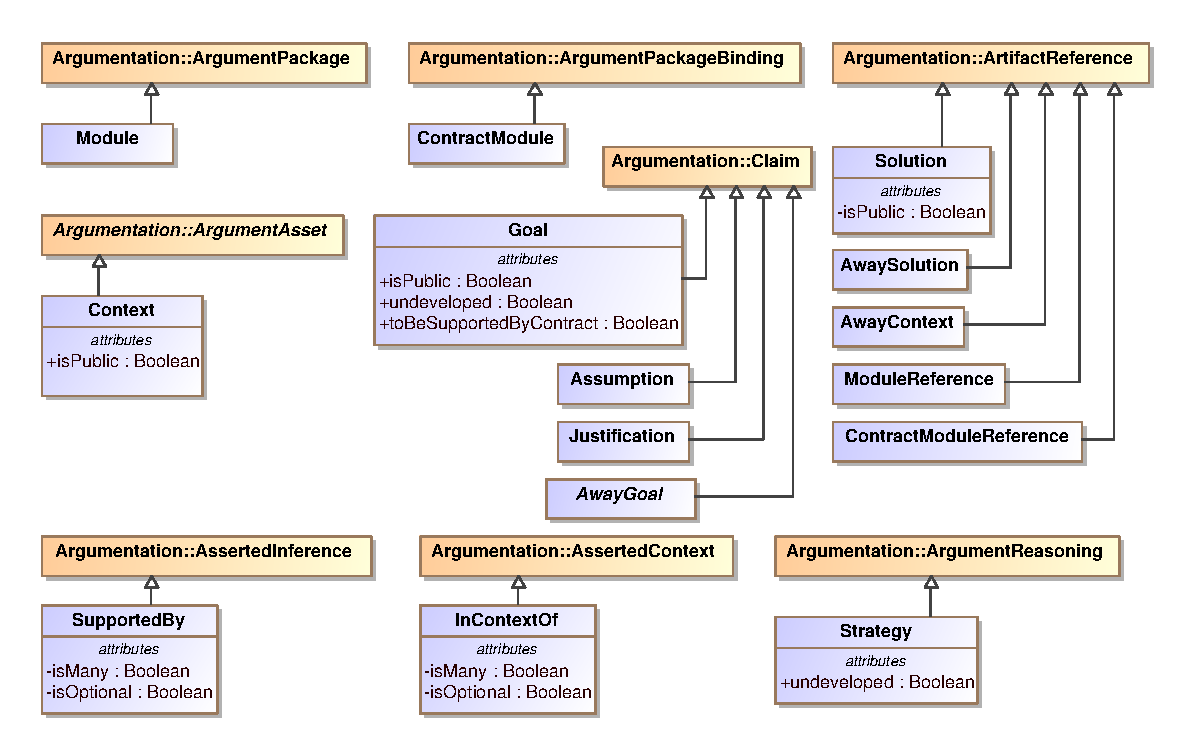
\includegraphics[width=1\linewidth]{GSN.eps}
	\caption{SACM compliant GSN metamodel.}
	\label{fig:gsnMetamodel}
\end{figure}

Our version of the GSN metamodel is shown in Figure~\ref{fig:gsnMetamodel}. In GSN, argumentations are organised in \textit{Module}s, which is made as a sub-type of \textit{ArgumentPackage} in SACM; \textit{ContractMoudle} are essentially contracts that binds \textit{Module}s together, thus it is a sub-type of \textit{ArgumentPackageBinding}. 

Elements \textit{Goal}, \textit{Assumption}, \textit{Justification} and \textit{AwayGoal} are made sub-types of \textit{Claim} in SACM. A \textit{Goal} can be \textit{uninstantiated}, which basically means it is abstract, this is captured by the \textit{+isAbstract} feature in SACM's \textit{SACMElement} class. A \textit{Goal} can be \textit{public}, which is deprecated in SACM, a \textit{Goal} can also be \textit{undeveloped} and \textit{toBeSupportedByContract}, which are captured individually. 

Elements \textit{Solution}, \textit{AwaySolution}, \textit{AwayContext}, \textit{ModuleReference} and \textit{ContractModuleReference} are sub-types of \textit{ArtifactReference} in SACM as they refer to artifacts that bears information they represent. \textit{Context} is a slightly complicated concept, as it can either be a statement stating the context of a \textit{Goal}, or it can refer to contextual information stored in an artifact. Thus, \textit{Context} is made a sub-type of \textit{ArgumentAsset}. 

\textit{SupportedBy} is made a sub-type of \textit{AssertedInference} and \textit{InContextOf} is made a sub-type of \textit{AssertedContext}. \textit{Strategy} is made a sub-type of \textit{ArgumentReasoning} for it explains the intention of an \textit{AssertedRelationship}.

The way that the GSN metamodel is created makes it inherently  
The reason that the GSN metamodel is created this way is that the created GSN metamodel also includes other packages in SACM, namely, the \textit{Base}, \textit{AssuranceCase}, \textit{Artifact} and \textit{Terminology} packages. Our vision is that such GSN metamodel is able to create